\documentclass[headings=optiontoheadandtoc,listof=totoc,parskip=full]{scrartcl}

\usepackage[tbtags]{amsmath,mathtools}
\usepackage{amssymb}
\usepackage{enumitem}
\usepackage[margin=.75in]{geometry}
\usepackage[headsepline]{scrlayer-scrpage}
\usepackage[USenglish]{babel}
\usepackage{hyperref}
\usepackage{graphicx}
\usepackage{float}
\usepackage{physics}
\usepackage[format=hang, justification=justified]{caption}
\usepackage{xcolor}
\usepackage{mathbbol}

\usepackage{cleveref} % Needs to be loaded last

\hypersetup{
	linktoc = all,
	pdfborder = {0 0 .5 [ 1 3 ]}
}

\def \reals {\mathbb{R}}
\DeclareMathOperator*{\argmax}{arg\,max}
\DeclarePairedDelimiter\floor{\lfloor}{\rfloor}

\pagestyle{scrheadings}
\rohead{Khedekar, Mangat \& Novotny}
\lohead{CS 479 Programming Assignment 3}

\title{Programming Assignment 3}
\subtitle{CS 479\\\url{https://github.com/alexander-novo/CS479-PA3}}
\author{Nikhil Khedekar\\33\%\\\Cref{sec:part-3} \and Mehar Mangat\\33\%\\\Cref{sec:part-3} \and Alexander Novotny\\33\%\\\Cref{sec:part-1}}
\date{Due: April 26, 2021 \\ Submitted: \today}

\begin{document}
\maketitle
\tableofcontents
\pagenumbering{gobble}

\newpage
\pagenumbering{arabic}

%%%%%%%%%%%%%%%%%%%%%%

\section{Theory}

This assignment considers the usage of Principal Component Analysis for dimensionality reduction for a dataset of images for the purpose of face recognition. 

\subsection{Principal Component Analysis (PCA)}
Principal Component Analysis (PCA) is a method for reducing the dimensionality of high dimensional data while preserving as much information as possible. The way this works is by the projection of the sample data along its principal distribution directions. Intuitively, this can be understood by finding the directions that capture the highest variance of the data and projecting the data along these directions. 


For some given sample data $\mathbf{X} = \{\vec x_i \in \reals^N, 1 \leq i \leq M\}$, where $M$ is the number of samples in the data set, the sample covariance matrix $\Sigma_x$ can be found using \cref{eq:mean} and \cref{eq:cov_mat}, where $\Bar{x}$ is the sample mean and $\Phi_i$ are the normalized data points:

\begin{equation} \label{eq:mean}
    \mathbf{\Bar{x}} = \frac{1}{M}\sum_{i = 1}^{M}\mathbf{x}_i
\end{equation}

\begin{equation}
    \mathbf{\Phi_i} = \mathbf{x}_i - \mathbf{\Bar{x}}
\end{equation}

\begin{equation} \label{eq:cov_mat}
    \mathbf{\Sigma_x} = \frac{1}{M}\sum_{i = 1}^M(\mathbf{x} - \mathbf{\Bar{x}})(\mathbf{x} - \mathbf{\Bar{x}})^T = \frac{1}{M}\sum_{i = 1}^{M}\mathbf{\Phi}_i\mathbf{\Phi}_i^T 
\end{equation}

\Cref{eq:cov_mat} can be further simplified to \cref{eq:cov_mat_simp} using \cref{eq:a_mat}.

\begin{equation}\label{eq:cov_mat_simp}
    \mathbf{\Sigma_x} = \frac{1}{M}\mathbf{A}\mathbf{A}^T
\end{equation}

\begin{equation}\label{eq:a_mat}
    \mathbf{A} = [\Phi_1 \Phi_2 ... \Phi_M]    
\end{equation}

The eigenvectors and eigenvalues of the covariance matrix have the special property that the eigenvectors form an orthogonal basis in $R^N$ for the sample data with the corresponding eigenvalues representing the variance of the data in these directions. The eigenvectors $\mathbf{u}_i$ and corresponding eigenvalues $\lambda_i$ are obtained using \cref{eq:eigenvec_and_eigenval}.

\begin{equation}\label{eq:eigenvec_and_eigenval}
    \mathbf{\Sigma_x}\mathbf{u_i} = \lambda_i\mathbf{u}_i
\end{equation}

In our notation, we assume that the eigenvalues are indexed in descending order, namely, $\lambda_1 > \lambda_2 > ... > \lambda_N$. Using the eigenvectors as the new basis we can represent our data samples $\mathbf{x} \in \reals^N$ by \cref{eq:eigenvec_rep}

\begin{equation}\label{eq:eigenvec_rep}
    \mathbf{x} - \mathbf{\Bar{x}} = \sum_{i = 1}^N \mathbf{y}_i\mathbf{u}_i = y_1\mathbf{u}_1 + y_2\mathbf{u}_2 + ... y_N\mathbf{u}_N
\end{equation}

where $y_1, y_2 ... y_N$ are the coefficients in this new basis and are given by \cref{eq:yi}.

\begin{equation}\label{eq:yi}
    y_i = \frac{(\mathbf{x} - \mathbf{\Bar{x}})^T \mathbf{u}_i}{\mathbf{u}_i\mathbf{u}_i^T} = (\mathbf{x} - \mathbf{\Bar{x}})^T\mathbf{\hat{u}}_i
\end{equation}

where $\mathbf{\hat{u}}_i$ represents the unit vector in the direction of $\mathbf{u}_i$. The final dimensionality reduction is carried out on the basis of \cref{eq:eigenvec_rep} in that only the components corresponding to the first $K (K << N)$ eigenvectors are kept and the remaining components are discarded. This formulation approximates $\mathbf{x}$ by $\mathbf{\hat{x}}$ for which \cref{eq:eigenvec_rep} can be rewritten as \cref{eq:eigenvec_rep_pc}.

\begin{equation}\label{eq:eigenvec_rep_pc}
    \mathbf{\hat{x}} - \mathbf{\Bar{x}} = \sum_{i = 1}^N \mathbf{y}_i\mathbf{u}_i = y_1\mathbf{u}_1 + y_2\mathbf{u}_2 + ... y_K\mathbf{u}_K
\end{equation}

\cref{eq:eigenvec_rep_pc} can be written in matrix form instead of the summation as \cref{eq:linear_transform_1}

\begin{equation}\label{eq:linear_transform_1}
    \mathbf{\hat{x}} - \mathbf{\Bar{x}} = \mathbf{U}\begin{bmatrix}y_1\\y_2\\...\\y_K\end{bmatrix}
\end{equation}

where $\mathbf{U} = [\mathbf{u}_1, \mathbf{u}_2, ... , \mathbf{u}_K]$ is an $N \times K$ matrix with its columns as the $K$ largest eigenvectors of the covariance matrix $\mathbf{\Sigma}_x$. \Cref{eq:linear_transform_1} can also be written as 

\begin{equation}\label{eq:linear_transform_2}
    \begin{bmatrix}y_1\\y_2\\...\\y_K\end{bmatrix} = \mathbf{U}^T(\mathbf{\hat{x}} - \mathbf{\Bar{x}})
\end{equation}

now represents each data sample as $x$  This can be re-written as a linear transformation as in 

\begin{equation}
    TODO
\end{equation}

\subsection{Eigenfaces and Facial Recognition}

The first widely successful method of solving the facial recognition problem is the eigenface method. An eigenface


\section{Implementation}
\section{Results and Discussion}

The calculated sample mean images for both data set can be found in \cref{fig:sample-means}. Note the appearance of a single pixel-wide border of dark pixels around both means - this seems to come from some sort of artifact in the original data sets consisting of slightly darker pixels on the border.

\begin{figure}[H]
	\centering
	\includegraphics[width=.4\textwidth]{../out/mean-H} \quad
	\includegraphics[width=.4\textwidth]{../out/mean-L}
	\caption{The sample mean face for the high resolution data set (left) and the low resolution data set (right).}
	\label{fig:sample-means}
\end{figure}

The 10 largest and smallest eigenfaces can be found in \cref{fig:largest-eigen-H,fig:largest-eigen-L}. Note that the largest eigenfaces all look like faces in some way, while the smallest eigenfaces might as well be random noise. This is a good justification for dimensionality reduction using PCA - these smallest eigenfaces are contributing very little meaningful data. Also note that each eigenface calculated from the low resolution data corresponds to one calculated from the high resolution data almost exactly. This makes sense, since the low resolution images are just sampled version of the high resolution images, so it would make sense that the principal components are just sampled version of the principle components of the high resolution images. Note that eigenfaces 7 and 8 correspond but are inverted between data sets - this is an example of how inverted eigenvectors are still eigenvectors.

\begin{figure}[H]
	\centering
	\includegraphics[width=.09\textwidth]{../out/eigenface-H-largest-1}
	\includegraphics[width=.09\textwidth]{../out/eigenface-H-largest-2}
	\includegraphics[width=.09\textwidth]{../out/eigenface-H-largest-3}
	\includegraphics[width=.09\textwidth]{../out/eigenface-H-largest-4}
	\includegraphics[width=.09\textwidth]{../out/eigenface-H-largest-5}
	\includegraphics[width=.09\textwidth]{../out/eigenface-H-largest-6}
	\includegraphics[width=.09\textwidth]{../out/eigenface-H-largest-7}
	\includegraphics[width=.09\textwidth]{../out/eigenface-H-largest-8}
	\includegraphics[width=.09\textwidth]{../out/eigenface-H-largest-9}
	\includegraphics[width=.09\textwidth]{../out/eigenface-H-largest-10}\\
	\includegraphics[width=.09\textwidth]{../out/eigenface-H-smallest-1}
	\includegraphics[width=.09\textwidth]{../out/eigenface-H-smallest-2}
	\includegraphics[width=.09\textwidth]{../out/eigenface-H-smallest-3}
	\includegraphics[width=.09\textwidth]{../out/eigenface-H-smallest-4}
	\includegraphics[width=.09\textwidth]{../out/eigenface-H-smallest-5}
	\includegraphics[width=.09\textwidth]{../out/eigenface-H-smallest-6}
	\includegraphics[width=.09\textwidth]{../out/eigenface-H-smallest-7}
	\includegraphics[width=.09\textwidth]{../out/eigenface-H-smallest-8}
	\includegraphics[width=.09\textwidth]{../out/eigenface-H-smallest-9}
	\includegraphics[width=.09\textwidth]{../out/eigenface-H-smallest-10}
	\caption{The 10 largest eigenfaces in decreasing order for the high resolution data set, followed by the 10 smallest eigenfaces in increasing order.}
	\label{fig:largest-eigen-H}
\end{figure}

\begin{figure}[H]
	\centering
	\includegraphics[width=.09\textwidth]{../out/eigenface-L-largest-1}
	\includegraphics[width=.09\textwidth]{../out/eigenface-L-largest-2}
	\includegraphics[width=.09\textwidth]{../out/eigenface-L-largest-3}
	\includegraphics[width=.09\textwidth]{../out/eigenface-L-largest-4}
	\includegraphics[width=.09\textwidth]{../out/eigenface-L-largest-5}
	\includegraphics[width=.09\textwidth]{../out/eigenface-L-largest-6}
	\includegraphics[width=.09\textwidth]{../out/eigenface-L-largest-7}
	\includegraphics[width=.09\textwidth]{../out/eigenface-L-largest-8}
	\includegraphics[width=.09\textwidth]{../out/eigenface-L-largest-9}
	\includegraphics[width=.09\textwidth]{../out/eigenface-L-largest-10}\\
	\includegraphics[width=.09\textwidth]{../out/eigenface-L-smallest-1}
	\includegraphics[width=.09\textwidth]{../out/eigenface-L-smallest-2}
	\includegraphics[width=.09\textwidth]{../out/eigenface-L-smallest-3}
	\includegraphics[width=.09\textwidth]{../out/eigenface-L-smallest-4}
	\includegraphics[width=.09\textwidth]{../out/eigenface-L-smallest-5}
	\includegraphics[width=.09\textwidth]{../out/eigenface-L-smallest-6}
	\includegraphics[width=.09\textwidth]{../out/eigenface-L-smallest-7}
	\includegraphics[width=.09\textwidth]{../out/eigenface-L-smallest-8}
	\includegraphics[width=.09\textwidth]{../out/eigenface-L-smallest-9}
	\includegraphics[width=.09\textwidth]{../out/eigenface-L-smallest-10}
	\caption{The same figure as \cref{fig:largest-eigen-H}, but for the low resolution data set.}
	\label{fig:largest-eigen-L}
\end{figure}

\begin{figure}[H]
	\centering
	\includegraphics[width=\textwidth]{../out/compare-80-90-95}
	\caption{A comparison of classification accuracy against number of images considered ($N$), the percentage of information preserved by eigenfaces, and the data set used.}
	\label{fig:classification-accuracy-H}
\end{figure}

\begin{figure}[H]
	\centering
	\includegraphics[width=.15\textwidth]{../Images/fb_H/01001_960627_fb}
	\includegraphics[width=.15\textwidth]{../Images/fb_H/00261_940128_fb}
	\includegraphics[width=.15\textwidth]{../Images/fb_H/00863_940307_fb}
	\quad
	\includegraphics[width=.15\textwidth]{../Images/fb_H/00556_940519_fb}
	\includegraphics[width=.15\textwidth]{../Images/fb_H/00212_940128_fb_a}
	\includegraphics[width=.15\textwidth]{../Images/fb_H/00695_941121_fb}\\
	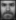
\includegraphics[width=.15\textwidth]{../Images/fa_H/01001_960627_fa}
	\includegraphics[width=.15\textwidth]{../Images/fa_H/00261_940128_fa}
	\includegraphics[width=.15\textwidth]{../Images/fa_H/00863_940307_fa}
	\quad
	\includegraphics[width=.15\textwidth]{../Images/fa_H/00557_940519_fa}
	\includegraphics[width=.15\textwidth]{../Images/fa_H/00266_940128_fa}
	\includegraphics[width=.15\textwidth]{../Images/fa_H/01005_960627_fa}
	\caption{High resolution testing images (top) and the training images they were matched against (bottom). Images which were correctly classified (i.e. both pictures are of the same subject) on the left, and incorrect classifications on the right.}
	\label{fig:classifications-H}
\end{figure}

\begin{figure}[H]
	\centering
	\includegraphics[width=.15\textwidth]{../Images/fb_L/01001_960627_fb}
	\includegraphics[width=.15\textwidth]{../Images/fb_L/00261_940128_fb}
	\includegraphics[width=.15\textwidth]{../Images/fb_L/00863_940307_fb}
	\quad
	\includegraphics[width=.15\textwidth]{../Images/fb_L/00770_960530_fb_a}
	\includegraphics[width=.15\textwidth]{../Images/fb_L/00212_940128_fb_a}
	\includegraphics[width=.15\textwidth]{../Images/fb_L/00695_941121_fb}\\
	\includegraphics[width=.15\textwidth]{../Images/fa_L/01001_960627_fa}
	\includegraphics[width=.15\textwidth]{../Images/fa_L/00261_940128_fa}
	\includegraphics[width=.15\textwidth]{../Images/fa_L/00863_940307_fa}
	\quad
	\includegraphics[width=.15\textwidth]{../Images/fa_L/00494_940519_fa}
	\includegraphics[width=.15\textwidth]{../Images/fa_L/00266_940128_fa}
	\includegraphics[width=.15\textwidth]{../Images/fa_L/00968_960627_fa}
	\caption{The same figure as \cref{fig:classifications-H}, but with images from the low resolution data set.}
	\label{fig:classifications-L}
\end{figure}

\begin{figure}[H]
    \centering
    \includegraphics[width=.75\textwidth]{../out/intruders}
    \caption{A comparison of intruder-detection ROC curves based on resolution.}
    \label{fig:intruders}
\end{figure}

\end{document}